\chapter{Automation Fundamentals for IT Consultants}


\section{Introduction}

As a small IT consulting firm, your time is your most valuable asset. In this chapter, we'll dive into the fundamental concepts of automation and explore how they can revolutionize your consulting practice. We'll start with a practical example that can save you hours each week and transform how you handle client communications.


\section{Understanding Automation in IT Consulting}

Automation in IT consulting refers to the use of technology to perform repetitive tasks, streamline processes, and reduce manual intervention. It's about working smarter, not harder.

\subsection{Key Benefits of Automation}

\begin{itemize}
    \item \textbf{Time Savings}: Automate repetitive tasks to focus on high-value activities.
    \item \textbf{Consistency}: Reduce human error and ensure consistent outcomes.
    \item \textbf{Scalability}: Handle increased workload without proportionally increasing resources.
    \item \textbf{Improved Client Satisfaction}: Faster response times and more accurate deliverables.
    \item \textbf{Data-Driven Insights}: Automated processes can generate valuable data for decision-making.
\end{itemize}

\begin{figure}[h]
    \centering
    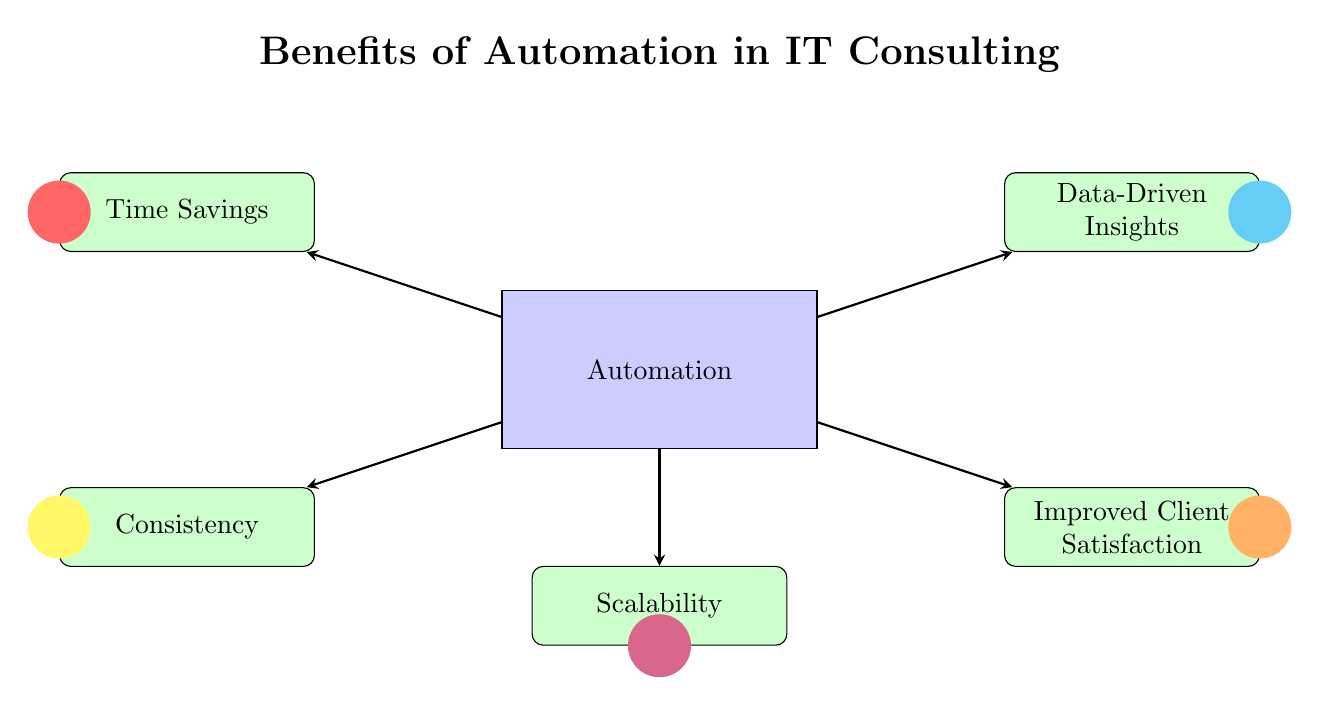
\begin{tikzpicture}
        [
        benefit/.style={rectangle, draw, fill=green!20, rounded corners, text width=3cm, align=center, minimum height=1cm},
        icon/.style={circle, fill=#1, minimum size=0.8cm},
        arrow/.style={->, >=stealth, thick}
        ]
        % Title
        \node[font=\Large\bfseries] (title) at (0,4) {Benefits of Automation in IT Consulting};

        % Central node
        \node[rectangle, draw, fill=blue!20, minimum width=4cm, minimum height=2cm, align=center] (automation) at (0,0) {Automation};

        % Benefit nodes
        \node[benefit] (time) at (-6,2) {Time Savings};
        \node[benefit] (consistency) at (-6,-2) {Consistency};
        \node[benefit] (scalability) at (0,-3) {Scalability};
        \node[benefit] (satisfaction) at (6,-2) {Improved Client Satisfaction};
        \node[benefit] (insights) at (6,2) {Data-Driven Insights};

        % Icons
        \node[icon=red!60] at (time.west) {};
        \node[icon=yellow!60] at (consistency.west) {};
        \node[icon=purple!60] at (scalability.south) {};
        \node[icon=orange!60] at (satisfaction.east) {};
        \node[icon=cyan!60] at (insights.east) {};

        % Arrows
        \draw[arrow] (automation) -- (time);
        \draw[arrow] (automation) -- (consistency);
        \draw[arrow] (automation) -- (scalability);
        \draw[arrow] (automation) -- (satisfaction);
        \draw[arrow] (automation) -- (insights);
    \end{tikzpicture}
    \caption{Benefits of Automation in IT Consulting}
    \label{fig:automation_benefits}
\end{figure}

\section{Types of Automation Relevant to IT Consulting}

\subsection{1. Process Automation}
Streamlining workflows and business processes. Examples include automated client onboarding or project management workflows.

\subsection{2. Data Automation}
Automating data collection, processing, and analysis. This could involve automated reporting or data migration tools.

\subsection{3. Communication Automation}
Automating client communications, notifications, and updates. Our email classification example falls under this category.

\subsection{4. Infrastructure Automation}
Automating the setup, configuration, and management of IT infrastructure. This includes automated server provisioning or network configuration.


\section{Quick Win: AI-Powered Email Classification with n8n and OpenAI}

Let's start with a common pain point: the overflowing inbox. We'll create an automation that reviews and classifies emails based on their content, helping you prioritize and respond more efficiently.

\subsection{Why This Matters}

\begin{figure}[h]
    \centering
    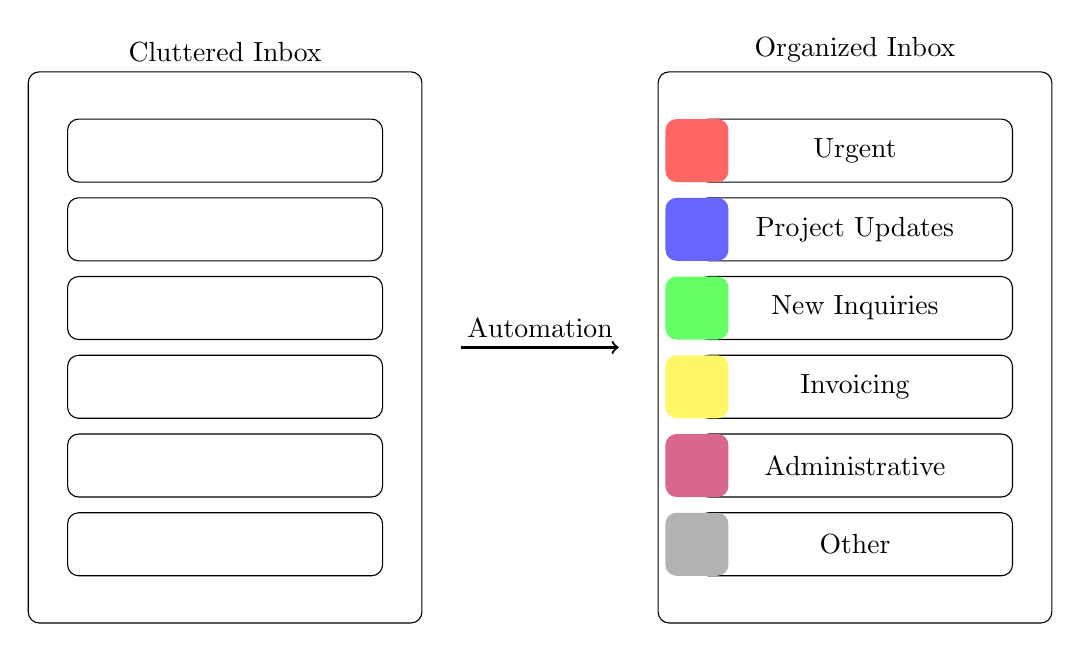
\begin{tikzpicture}[
        inbox/.style={rectangle, draw, rounded corners, minimum width=5cm, minimum height=7cm},
        email/.style={rectangle, draw, rounded corners, fill=white, minimum width=4cm, minimum height=0.8cm},
        label/.style={rectangle, rounded corners, fill=#1, minimum width=0.8cm, minimum height=0.8cm},
    ]
        % Cluttered Inbox
        \node[inbox] (cluttered) at (0,0) {};
        \node[above] at (cluttered.north) {Cluttered Inbox};
        \foreach \y in {2.5,1.5,0.5,-0.5,-1.5,-2.5} {
            \node[email] at (0,\y) {};
        }

        % Arrow
        \draw[->,thick] (3,0) -- (5,0) node[midway,above] {Automation};

        % Organized Inbox
        \node[inbox] (organized) at (8,0) {};
        \node[above] at (organized.north) {Organized Inbox};

        % Classified emails
        \node[email] (urgent) at (8,2.5) {Urgent};
        \node[label=red!60] at (urgent.west) {};

        \node[email] (project) at (8,1.5) {Project Updates};
        \node[label=blue!60] at (project.west) {};

        \node[email] (inquiry) at (8,0.5) {New Inquiries};
        \node[label=green!60] at (inquiry.west) {};

        \node[email] (invoice) at (8,-0.5) {Invoicing};
        \node[label=yellow!60] at (invoice.west) {};

        \node[email] (admin) at (8,-1.5) {Administrative};
        \node[label=purple!60] at (admin.west) {};

        \node[email] (other) at (8,-2.5) {Other};
        \node[label=gray!60] at (other.west) {};
    \end{tikzpicture}
    \caption{Cluttered inbox vs. Organized, classified inbox}
    \label{fig:inbox_comparison}
\end{figure}

Imagine starting your day with a perfectly organized inbox, where emails are automatically sorted into categories like:

\begin{itemize}
    \item Urgent client issues
    \item Project updates
    \item New business inquiries
    \item Invoicing and payments
    \item Administrative tasks
\end{itemize}

This automation will make that a reality, allowing you to:
\begin{itemize}
    \item Respond to critical issues faster
    \item Prioritize your workday more effectively
    \item Ensure no important client communication slips through the cracks
\end{itemize}

Here's going to be our flow:

\begin{figure}
    \centering
    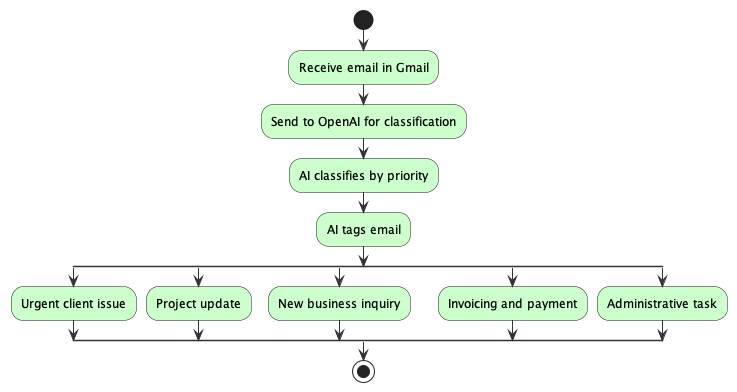
\includegraphics[width=0.8\textwidth]{./figures/01-n8n-flow}
    \caption{Email Classification and Tagging Automation Flow}
    \label{fig:01_email_automation}
\end{figure}


\section{Setting Up Your Secure Automation Environment}

Before we dive into the automation itself, let's set up n8n locally. Unlike cloud-based tools like Zapier, n8n can be self-hosted, ensuring your sensitive client data never leaves your control.

\subsection{Installing n8n using Docker}

We'll use Docker for a consistent setup across all platforms.

\begin{enumerate}
    \item Install Docker:
    \begin{itemize}
        \item For Windows: Docker Desktop for Windows
        \item For macOS: Docker Desktop for Mac
        \item For Linux: Docker Engine
    \end{itemize}
    \item With Docker installed, open a terminal or command prompt and run:
    \begin{lstlisting}[language=bash, label={lst:n8n-docker-run}]
docker run -it --rm \
  --name n8n \
  -p 5678:5678 \
  -v ~/.n8n:/home/node/.n8n \
  n8nio/n8n
    \end{lstlisting}
    \item Open your browser and navigate to \url{http://localhost:5678}
    \item Complete the setup process
\end{enumerate}

% TODO @screenshot: n8n setup screen


\section{Creating Your Email Classification Workflow}

Now that n8n is running, let's build our automation:

\subsection{Step 1: Connect to Gmail}

\begin{enumerate}
    \item In n8n, add a new "Gmail" node and select "On New Email"
    \item Follow the OAuth process to connect your Gmail account
\end{enumerate}

% TODO @screenshot: Gmail node configuration in n8n

\subsection{Step 2: Integrate OpenAI for Content Analysis}

\begin{enumerate}
    \item Add an "OpenAI" node
    \item Configure it to use the GPT-3 model for text classification
    \item Set up the prompt to classify the email content
\end{enumerate}

% TODO @screenshot: OpenAI node configuration in n8n

\subsection{Step 3: Update Email Labels}

\begin{enumerate}
    \item Add another "Gmail" node
    \item Configure it to add a label based on the classification from OpenAI
\end{enumerate}

% TODO @screenshot: Final Gmail node configuration for labeling


\section{Testing and Refining Your Workflow}

\begin{enumerate}
    \item Use n8n's built-in testing features to run your workflow with sample emails
    \item Adjust the OpenAI prompt or classification categories as needed
    \item Monitor the workflow's performance over time and make refinements
\end{enumerate}


\section{Security Considerations}

When working with email automation, security is paramount. Here are some key considerations:

\begin{itemize}
    \item Use OAuth for secure authentication with Gmail
    \item Regularly review and rotate API keys for OpenAI
    \item Implement error handling to prevent sensitive data leaks
    \item Regularly audit your workflow's access and permissions
\end{itemize}


\section{Scaling Your Email Automation}

As your consulting practice grows, you can enhance this automation:

\begin{itemize}
    \item Implement more sophisticated classification logic
    \item Integrate with your CRM to update client records automatically
    \item Create automated responses for common inquiries
    \item Extend the workflow to handle multiple email accounts
\end{itemize}


\section{Real-World Impact: A Case Study}

Meet Sarah, a solo IT consultant. Before implementing this automation, Sarah spent 2 hours each day sorting through emails. After setting up the AI-powered classification:

\begin{itemize}
    \item Sarah's email processing time dropped to 30 minutes a day
    \item Her response time to urgent client issues improved by 60\%
    \item She never missed a new business inquiry, increasing potential leads by 25\%
\end{itemize}

By reclaiming 7.5 hours each week, Sarah was able to take on two additional clients without hiring help.


\section{Conclusion}

This email classification automation is just the tip of the iceberg. As you become more comfortable with n8n and other automation tools, you'll find countless opportunities to streamline your consulting practice. In the next chapter, we'll explore more advanced automation techniques and how to integrate them into your core services.

\textbf{Action Items:}
\begin{enumerate}
    \item Set up the email classification workflow we've created
    \item Run the workflow for a week and measure the time saved
    \item Identify two other repetitive tasks in your practice that could benefit from automation
\end{enumerate}

Remember, automation is a journey, not a destination. Start with this email classification workflow, then explore how you can automate other aspects of your consulting practice.

% TODO @qr: QR code linking to additional n8n tutorials and resources